%%%% Dokumentklassen %%%%

\documentclass[a4paper,11pt,fleqn,dvipsnames,oneside,openany]{memoir} 	% Openright åbner kapitler på højresider (openany begge)



%%%% PACKAGES %%%%

%% Oversættelse og tegnsætning %%
\usepackage[utf8]{inputenc}					% Input-indkodning af tegnsæt (UTF8)
\usepackage[danish]{babel}					% Dokumentets sprog
\usepackage[T1]{fontenc}					    % Output-indkodning af tegnsæt (T1)
\usepackage{ragged2e,anyfontsize}			% Justering af elementer
\usepackage{fixltx2e}						% Retter forskellige fejl i LaTeX-kernen

\usepackage{lastpage}						% Total antal sider opdateres automatisk ved \pageref{LastPage}
																			
%% Figurer og tabeller (floats) %%
\usepackage{graphicx} 						% Håndtering af eksterne billeder (JPG, PNG, EPS, PDF)
\usepackage{multicol}         	            	% Muliggør output i spalter
\usepackage{rotating}						% Rotation af tekst med \begin{sideways}...\end{sideways}
\usepackage{xcolor}							% Definer farver med \definecolor. Se mere: http://en.wikibooks.org/wiki/LaTeX/Colors
\usepackage{flafter}						% Sørger for at floats ikke optræder i teksten før deres reference
\let\newfloat\relax 						% Justering mellem float-pakken og memoir
\usepackage{float}							% Muliggør eksakt placering af floats, f.eks. \begin{figure}[H]

%% Matematik mm. %%
\usepackage{amsmath,amssymb,stmaryrd} 		% Avancerede matematik-udvidelser
\usepackage{mathtools}						% Andre matematik- og tegnudvidelser
\usepackage{textcomp}                 		% Symbol-udvidelser (fx promille-tegn med \textperthousand)
\usepackage{rsphrase}						% Kemi-pakke til RS-saetninger, fx \rsphrase{R1}
\usepackage[version=3]{mhchem} 				% Kemi-pakke til flot og let notation af formler, f.eks. \ce{Fe2O3}
\usepackage{siunitx}						% Flot og konsistent præsentation af tal og enheder med \si{enhed} og \SI{tal}{enhed}
\sisetup{output-decimal-marker = {,}}		% Opsætning af \SI (DE for komma som decimalseparator) 

%% Referencer og kilder %%
\usepackage[danish]{varioref}				% Muliggør bl.a. krydshenvisninger med sidetal (\vref)
%\usepackage{natbib}							% Udvidelse med naturvidenskabelige citationsmodeller

\usepackage[backend=bibtex, maxnames=1, url=false, style=science, natbib=true]{biblatex}
\addbibresource{Bibliografi/Ref.bib}


\usepackage{xr}							    % Referencer til eksternt dokument med \externaldocument{<NAVN>}

%% Misc. %%
\usepackage{listings}						% Placer kildekode i dokumentet med \begin{lstlisting}...\end{lstlisting}
\usepackage{lipsum}							% Dummy text \lipsum[..]
\usepackage[shortlabels]{enumitem}			% Muliggør enkelt konfiguration af lister
\usepackage{pdfpages}						% Gør det muligt at inkludere pdf-dokumenter med kommandoen \includepdf[pages={x-y}]{fil.pdf}	
\pdfoptionpdfminorversion=6					% Muliggør inkludering af pdf-dokumenter, af version 1.6 og højere
\pretolerance=2500 							% Justering af afstand mellem ord (højt tal, mindre orddeling og mere luft mellem ord)


%%%% CUSTOM SETTINGS %%%%

%% Marginer %%
\setlrmarginsandblock{2.5cm}{2.5cm}{*}		% \setlrmarginsandblock{Indbinding}{Kant}{Ratio}
\setulmarginsandblock{2.5cm}{3.0cm}{*}		% \setulmarginsandblock{Top}{Bund}{Ratio}
\checkandfixthelayout 						% Oversætter værdier til brug for andre pakker

%% Afsnitsformatering %%
\setlength{\parindent}{0mm}           		% Størrelse af indryk
\setlength{\parskip}{3mm}          			% Afstand mellem afsnit ved brug af double Enter
\linespread{1,1}							% Linjeafstand

%% Indholdsfortegnelse %%
\setsecnumdepth{subsection}		 			% Dybden af nummererede overskrifter (part/chapter/section/subsection)
\maxsecnumdepth{subsection}					% Dokumentklassens grænse for nummereringsdybde
\settocdepth{subsection} 					% Dybden af indholdsfortegnelsen
		
%% Opsætning af listings %%
\definecolor{commentGreen}{RGB}{34,139,24}
\definecolor{stringPurple}{RGB}{208,76,239}

\lstset{language=Matlab,					    % Sprog
	basicstyle=\ttfamily\scriptsize,		    % Opsætning af teksten
	keywords={for,if,while,else,elseif,		% Nøgleord at fremhæve
			  end,break,return,case,
			  switch,function},
	keywordstyle=\color{blue},				% Opsætning af nøgleord
	commentstyle=\color{commentGreen},		% Opsætning af kommentarer
	stringstyle=\color{stringPurple},		% Opsætning af strenge
	showstringspaces=false,					% Mellemrum i strenge enten vist eller blanke
	numbers=left, numberstyle=\tiny,		    % Linjenumre
	extendedchars=true, 					    % Tillader specielle karakterer
	columns=flexible,						% Kolonnejustering
	breaklines, breakatwhitespace=true,		% Bryd lange linjer
}

%% Navngivning %%
\addto\captionsdanish{
	\renewcommand\appendixname{Appendiks}
	\renewcommand\contentsname{Indholdsfortegnelse}	
	\renewcommand\appendixpagename{Appendiks}
	\renewcommand\appendixtocname{Appendiks}
	\renewcommand\cftchaptername{\chaptername~}		% Skriver "Kapitel" foran kapitlerne i indholdsfortegnelsen
	\renewcommand\cftappendixname{\appendixname~}	% Skriver "Appendiks" foran appendiks i indholdsfortegnelsen
}

%% Kapiteludssende %%
\definecolor{numbercolor}{gray}{0.7}		            % Definerer en farve til brug til kapiteludseende
\newif\ifchapternonum

\makechapterstyle{jenor}{					        % Definerer kapiteludseende frem til ...
  \renewcommand\beforechapskip{0pt}
  \renewcommand\printchaptername{}
  \renewcommand\printchapternum{}
  \renewcommand\printchapternonum{\chapternonumtrue}
  \renewcommand\chaptitlefont{\fontfamily{pbk}\fontseries{db}\fontshape{n}\fontsize{25}{35}\selectfont\raggedleft}
  \renewcommand\chapnumfont{\fontfamily{pbk}\fontseries{m}\fontshape{n}\fontsize{1in}{0in}\selectfont\color{numbercolor}}
  \renewcommand\printchaptertitle[1]{%
    \noindent
    \ifchapternonum
    \begin{tabularx}{\textwidth}{X}
    {\let\\\newline\chaptitlefont ##1\par} 
    \end{tabularx}
    \par\vskip-2.5mm\hrule
    \else
    \begin{tabularx}{\textwidth}{Xl}
    {\parbox[b]{\linewidth}{\chaptitlefont ##1}} & \raisebox{-15pt}{\chapnumfont \thechapter}
    \end{tabularx}
    \par\vskip2mm\hrule
    \fi
  }
}											        % ... her

\chapterstyle{jenor}						        % Valg af kapiteludseende - Google 'memoir chapter styles' for alternativer

%% Sidehoved %%

\makepagestyle{AAU}							        % Definerer sidehoved og sidefod udseende frem til ...
\makepsmarks{AAU}{%
	\createmark{chapter}{left}{shownumber}{}{. \ }
	\createmark{section}{right}{shownumber}{}{. \ }
	\createplainmark{toc}{both}{\contentsname}
	\createplainmark{lof}{both}{\listfigurename}
	\createplainmark{lot}{both}{\listtablename}
	\createplainmark{bib}{both}{\bibname}
	\createplainmark{index}{both}{\indexname}
	\createplainmark{glossary}{both}{\glossaryname}
}
\nouppercaseheads									% Ingen Caps ønskes

\makeevenhead{AAU}{\small ST3PRJ3 Gruppe 2}{}{\leftmark}	% Definerer lige siders sidehoved (\makeevenhead{Navn}{Venstre}{Center}{Hoejre})
\makeoddhead{AAU}{\rightmark}{}{\small ASE}		            % Definerer ulige siders sidehoved (\makeoddhead{Navn}{Venstre}{Center}{Højre})
\makeevenfoot{AAU}{\small \thepage}{}{}						% Definerer lige siders sidefod (\makeevenfoot{Navn}{Venstre}{Center}{Højre})
\makeoddfoot{AAU}{}{}{\small \thepage}						% Definerer ulige siders sidefod (\makeoddfoot{Navn}{Venstre}{Center}{Højre})

\copypagestyle{AAUchap}{AAU}							% Sidehoved for kapitelsider defineres som standardsider, men med blank sidehoved
\makeoddhead{AAUchap}{}{}{}
\makeevenhead{AAUchap}{}{}{}
\makeheadrule{AAUchap}{\textwidth}{0pt}
\aliaspagestyle{chapter}{AAUchap}					% Den ny style vælges til at gælde for chapters
													% ... her
															
\pagestyle{AAU}										% Valg af sidehoved og sidefod


%%%% CUSTOM COMMANDS %%%%

%% Billede hack %%
\newcommand{\figur}[4]{
		\begin{figure}[H] \centering
			\includegraphics[width=#1\textwidth]{billeder/#2}
			\caption{#3}\label{#4}
		\end{figure} 
}

%% Specielle tegn %%
\newcommand{\decC}{^{\circ}\text{C}}
\newcommand{\dec}{^{\circ}}
\newcommand{\m}{\cdot}


%%%% ORDDELING %%%%

\hyphenation{}


%%%% Tilføjelser af min preample %%%%

% Booktabs:
% The booktabs package is needed for better looking tables. 
\usepackage{booktabs}

% Caption:
% For better looking captions. See caption documentation on how to change the format of the captions.
\usepackage[hang, font={small, it}]{caption}

% Hyperref:
% This package makes all references within your document clickable. By default, these references will become boxed and colored. This is turned back to normal with the \hypersetup command below.
\usepackage{hyperref}
	\hypersetup{colorlinks=false,pdfborder=0 0 0}

% Cleveref:
% This package automatically detects the type of reference (equation, table, etc.) when the \cref{} command is used. It then adds a word in front of the reference, i.e. Fig. in front of a reference to a figure. With the \crefname{}{}{} command, these words may be changed.
\usepackage{cleveref}
	\crefname{equation}{formel}{formler}
	\crefname{figure}{figur}{figurer}	
	\crefname{table}{tabel}{tabeller}

% Mine tilføjelser:
\usepackage{units}                        %% Bruges til at gøre fx 1/2 samlet med: \nicefrac{1}{2}.
\usepackage{tabu, longtable}              %% Bruges til tabeller.
\setlength{\tabulinesep}{1.5ex}           %% Definerer linjeafstand i tabeller.
\usepackage{enumerate}                    %% Bruges til lister.
\usepackage{tabto}                        %% Giver mulighed for TAB med fx \tabto{3em}.
\usepackage[hyphenbreaks]{breakurl}       %% Bruges til websiders url'er.
\renewcommand{\UrlFont}{                  %% Definerer url-font.
\small\ttfamily}                          %
%\bibliographystyle{unsrt}                 %% Definere bibliografien. Ses til sidst i dokumentet i kapitlet Litteratur.
\usepackage{amssymb} 
\usepackage{pifont}
%\newcommand{\xmark{\ding{55}}			 % Opretter et unchecked mark
\usepackage{url}

\usepackage{pifont}
\usepackage{nccmath}						% Bruges til centering af equations (\begin{ceqn})



\usepackage{url}
\usepackage{hyperref}
%\usepackage{natbib}
%\bibliographystyle{plainnat}
%\usepackage{biblatex}

\raggedbottom

%\externaldocument[D-]{Dokumentation}

\begin{document}

	
\frontmatter						% Nummereres med romerske tal.
\let\cleardoublepage\clearpage
\begin{titlingpage}
\begin{center}
~ \\[3cm]


\includegraphics[width=0.6\textwidth]{figurer/ASE}~\\[1cm]

\textsc{\LARGE Aarhus School of Engineering}\\[1.5cm]

\textsc{\Large Sundhedsteknologi}\\
\textsc{\Large Medicinsk Teknologi Vurdering }\\[0.5cm]

\noindent\makebox[\linewidth]{\rule{\textwidth}{0.4pt}}\\
[0.5cm]{\Huge Ultralyds Robotarm}
\noindent\makebox[\linewidth]{\rule{\textwidth}{0.4pt}}

\end{center}

Anne Bundgaard Hoelgaard\tab(201404492) \newline
Ditte Heebøll Callesen\tab(201408392) \newline
Freja Ramsing Munk\tab(2014) \newline
Ida Mark Skovbjerg\tab(2014) \newline	
Mette Østergård Knudsen\tab(2014) \newline 
Nina Brkovic\tab(2014) \newline 


\textit{Vejledere:} \newline
Lene Hause\\
Samuel Alberg Thrysøe
Aarhus Universitet

\vfill

\begin{center}
{\large 16. december 2015}
\end{center}

\end{titlingpage}
\chapter{Abstract} 
\subsubsection{Introduction}
Sonographers who work with ultrasonic examination of pregnant women are at risk of getting work-related disorder due to poor work postures. It is often necessary to press the ultrasonic probe against the stomach, while the probe is being held at arm’s length. An Ultrasonic Robotic Arm will reduce the amount of poor work postures. The Robotic Arm where the ultrasonic probe is attached will be controlled by the sonographer with a joystick. The sonographer thereby avoids the previously mentioned physical challenges and potential discomforts. 

\subsubsection{Methods}
The purpose of this report has been to study which consequences the implementation of the Ultrasonic Robotic Arm can have with focus on four perspectives: Technology, Organization, Patient, and Economics. 
Information which can be used in all perspectives has been obtained through interviews with departments for ultrasonic examinations of pregnant women in the Regional Hospital of Horsens and the Regional Hospital of Viborg. Specific methods has been used for each perspective.

\subsubsection{Discussion}
This report is based on a summary of interviews, scientific articles, and assumptions. This is partly because the Ultrasonic Robotic Arm is not fully developed, which causes an insecurity which could have been reduced throughout other researches. 
The Ultrasonic Robotic Arm can be used as equipment for telemedicine in the future. This will require an attachment of a camera and a microphone to the system. There will be no direct changes to the Ultrasonic Robotic Arm. The sonographer does not need to be in the same room as the pregnant woman during the ultrasonic examination. 

\subsubsection{Conclusion} 
The Ultrasonic Robotic Arm will be able to reduce the amount of work-related disorder and poor work postures for sonographers during ultrasonic examination of pregnant women. The sonographers will be able to perform ultrasonic examinations 37 hours a week and stay in the job for a greater amount of years. The Robotic Arm will not lead to changes for the patient with regard to the quality and the result of the ultrasonic examination. 
The Ultrasonic Robotic Arm has a technological restriction, which means it can be used for 70-80\% of the ultrasonic examinations of pregnant women. The remaining 20-30\% of the ultrasonic examinations must be performed manually. From an economic perspective savings in wage costs will not cover the annual depreciation provision on the purchase of the Ultrasonic Robotic Arm.



\chapter{Resumé}

%\begin{figure}[h!]\centering
%	\includegraphics[width = 0.4\textwidth]{Filnavn}
%	\caption{Billede 1}
%	\label{billede1}
%\end{figure}
\chapter{Forord}
Denne mini-MTV er udarbejdet på 4. semester på Sundhedsteknologi, Aarhus Universitet Ingeniørhøjskolen (IHA), under vejledning af Lene Häuser Petersen og Samuel Alberg Thrysøe. Projektet tager sit udgangspunkt i undervisningen på IHA, og udspringer fra kurset Medicinsk Teknologi Vurdering. 


I forbindelse med udformningen af denne mini Medicinsk Teknologi Vurdering vil vi gerne takke følgende personer og afdelinger, for deres venlighed og hjælp:


Tak til Tina Arnbjørn fra Hospitalsenheden Horsens, Kvindeafdelingen, Svangre- og Ultralydsambulatorium for at stille op til interview, og tak til afdelingen for demonstrering af ultralydsscanninger. 


Tak til Karen Marie Goul fra Regionshospital Midt Viborg, Kvindesygdomme og Fødsler for at stille op til interview. Samt et tak til afdelingen for demonstrationer af ultralydsscanninger. 


Endvidere skal der lyde en stor tak til Søren Pallesen for idegrundlag, hans viden omkring Ultralyds Robotarmen, samt inspiration til litteratursøgning. 


\chapter{Forkortelser og formler}

\section{Forkortelser}
\begin{longtabu} to \linewidth{@{}l X[j]@{}}
    Ord &    Forklaring\\
    \toprule\ \\
    Robotarm & Ultralyds robotarm udviklet af Robotic Ultrasound ApS \\
    MTV & Medicinsk Teknologi Vurdering \\
  	RMV & Regionshospital Midt Viborg, Kvindesygdomme og Fødsler \\
  	HEH & Hospitalsenheden Horsens, Kvindeafdelingen, Svangre- og Ultralydsambulatorium \\
  	BMI & Body Mass Index \\
  	Bilag 12, 28.04.2016 & Se bilag 12 under dato 28.04.2016
   
\label{forkort}
\end{longtabu}

\section{Formler} \label{Formler}
Annunitetsmetoden: \\
Viser den gennemsnitlige årlige værdi af en investering. Baseret på den forventede levetid og en pålagt årlig rente.
\begin{equation}
\left( \dfrac{(1+\text{rente})^{\text{forventet levetid}}\cdot \text{rente}}{(1+\text{rente})^{\text{forventet levetid}}-1}\right)\cdot \text{udstyrspris} = \text{gennemsnitlige årlige værdi}
\end{equation}
\chapter{Formler}


%\cleardoublepage	
	
%\tableofcontents*                   % Indsætter en indholdsfortegnelse før Indledning.
%\addcontentsline{toc}{List of Figures}	%Tilføjer liste af figurer i indholdsfortegnelsen. 

\mainmatter                         % Her findes de nummererede kapitler modsat \frontmatter og \backmatter. Nummereres med arabiske tal.

\chapter{Indledning} 
Ved ultralydsscanning af gravide er arbejdsgener (og -skader) hos sonograferne et kendt problem. For at udføre scanningerne holder sonograferne proben i akavede stillinger, der udsætter deres skulder, arm og håndled for store belastninger \textbf{(reference)}. Hvilket blot forøges når et pres på mellem 3 og 11 kg. kræves for at få et klart ultralydsbillede \textbf{(reference til Søren)}. Disse stillinger øger risikoen for at få arbejdsskader. Grundet sonografernes belastende arbejdsstillinger er der fra Dansk Føtalmedicinsk Selskab udstukket guidelines angående det maksimale antal timer, en sonograf anbefales at foretage scanninger i løbet af en uge. Disse guidelines er på 28 timer om ugen \textbf{(reference)}. Dette gør at der skal flere sonografer til for at kunne scanne det stigende antal gravide i Danmark.\cite{Foedsler}. \\
Samtidig er Danmark inde i en udvikling, der gør at antallet af overvægtige stiger \cite{Overvaegt}. Dette gør at sonograferne skal presse med en større kraft for at få billeder af tilsvarende kvalitet frem. 

Gennem en årrække er der lavet en række forskningsstudier og forsøg med robotarm til ultralydsscanning af hjertet \textbf{(reference – artikel 8)}. Dette er med til at underbygge, at problemstillingen er kendt, men samtidig også at den optimale metode endnu ikke er fundet. Yderligere findes der flere forskningsstudier der drejer sig om udviklingen af robotter til lignende opgaver \textbf{(reference)}. Dette viser, at det er et område der investeres penge i og hvor der er en tro på at der er en fremtid i. 

Denne udvikling har ført til, at firmaet Robotic Ultrasound ApS er i færd med at udvikle en Ultralyds Robotarm, der formodentlig kan afhjælpe problemet. Denne robotarm styres via et joystick, således at sonograferne kan undgå at være i de akavede arbejdsstillinger, men i stedet kan styre robotten til de ønskede stillinger. 

%Problemstillingen i denne form er et område der ikke tidligere er afdækket. Men tidligere forskning i forhold til ultralydsscanning med robot gør at der findes tilstrækkelig videnskabelig dokumentation til at bygge mini-MTV’en op omkring. 

\section{Formål}
Formålet med denne mini-MTV er derfor at vurderer om Ultralyds Robotarmen kan implementeres som en teknologisk aflastnings løsning for sonografer i deres arbejde med scanning af gravide. Det ønskes at klarlægge fordele og ulemper ved både de eksisterende arbejdsforhold, og forholdene ved implementering af Ultralyds Robotarmen, samt hvilke forskelle robotarmen vil medføre for sonografer og gravide.

Yderligere forventes det, at rapportens resultater vil blive efterspurgt forud for en beslutningstagning når robotarmen er færdigudvikler og produceret. Dermed er formålet med mini-MTV’en også at bidrage til beslutningsgrundlaget for den enkelte sygehusafdeling, om Ultralyds Robotarmen skal implementeres, og i så fald hvilke aspekter der skal tages højde for og medtages i en vurdering. \textbf{Reference til metodehåndbog??}

\section{Projektafgrænsning}
Projektet afgrænses til en vurdering af, hvorvidt det kan betale sig at gøre brug af en Ultralyds Robotarm ved scanning af gravide i forhold til det udstyr der benyttes på afdelingerne i dag. Det primære fokus i projektet er problemstillingen om, at et stort antal sonografer oplever arbejdsskader og -gener ved scannings arbejdet \textbf{(reference)}. 

Ultralyds robotarmen åbner også for muligheden om, at bruge denne som en telemedicinsk løsning, hvor selve sonografen der foretager scanningen er placeret på et andet sygehus. Dette aspekt er det fravalgt at vurdere på i denne mini-MTV. 

Opgaven er afgrænset til at en 25 siders rapport, hvor det skriftlige omfang på en typisk dansk MTV ligger på over 100 sider. Dette gør, at det er en mini-MTV der udarbejdes. I en mini-MTV vurderes problemstillingen på de fire parametre: \textit{organisation, patient, teknologi og økonomi.} 

Den korte tidshorisont til udarbejdelsen af denne mini-MTV har været en afgørende faktor for, at det er valgt at begrænse projektet til at bygge på interview med to relevante danske sygehus afdelinger, samt en litteratursøgning på problemstillingen. Normalt er udarbejdelsen af en MTV en lang proces, da det kræver stort researcharbejde. Interview er afholdt med ”Kvindeafdelingen, Svangre- og Ultralydsambulatorium” på Hospitalsenheden Horsens (HEH) og afdelingen ”Kvindesygdomme og Fødsler” på Regionshospitalet Viborg (RMV).

\section{Projektorganisation}
Projektet er blevet udarbejdet som semesterprojekt af seks sundhedsteknologistuderende på 4. semester ved Ingeniørhøjskolen Aarhus Universitet. De studerende har været i en projektgruppe. \\
Hovedforfattere til de enkelte kapitlerne er:
\begin{itemize}
\item \textit{Organisation: }Anne Hoelgaard, Ida Skovbjerg og Nina Brkovic
\item \textit{Patient: }Ditte Callesen, Nina Brkovic og Freja Munk
\item \textit{Teknologi: }Ida Skovbjerg, Ditte Callesen og Mette Knudsen
\item \textit{Økonomi: }Anne Hoelgaard, Freja Munk og Mette Knudsen
\end{itemize}

\label{version_Systemark}
%\end{longtabu}
\chapter{Metoder}
Afsnittet indeholder en beskrivelse af hvilke metoder, der er blevet anvendt til udarbejdelse af denne mini-MTV i forhold til de fire MTV aspekter: Teknologi, Patient, Organisation og Økonomi.

Overordnet set er der blevet gennemført en litteratursøgning og -vurdering på baggrund af en i forvejen opstillet protokol (Bilag xx). Protokollen er udarbejdet ud fra specifikke søgestrategier, hvor der er søgt på både engelsk og dansk. De specifikke søgeord er medtaget som dokumentation. Der er søgt i følgende databaser: Embase, PubMed, Google Scholar, Cochrane og Engineering Village. \\
De fremsøgte artikler er blevet sorteret ud fra inklusions- og eksklusionskriterier. Artikler, som omhandlede specifikt telemedicin er blevet ekskluderet, da indholdet ikke er relevant for problemstillingen. Artikler omhandlende scanning af gravide, scanning af hjertet, robotarm og arbejdsskader hos sonografer er inkluderet i mini-MTV’en.\\
Udover ovenstående litteratur er der, efter behov søgt efter ikke videnskabelig litteratur for at opnå en forståelse for opbygningen af sonograf uddannelse, ultralydsscanning og andre løse emner for at komme ind i problemstillingen. 

\section{Teknologi}
Dataindsamling til Teknologiafsnittet er sket via antagelser fra CEO Søren Pallesen, Robotic Ultrasound ApS og produktspecifikationer fra Universal Robots, samt information fra interview og samtale med sonografer på HEH og RVM. Afsnittet belyser Ultralyds Robotarmens anvendelsesområder, specifikationer samt sikkerhedsindstillinger.
\section{Patient}
Patientafsnittet bygger på data fra interview og samtale med sonografer på HEH, samt viden fra etik undervisning. Derudover er de fem patientperspektiver – sociale, økonomiske, etiske, individuelle og kommunikative forhold – blevet benyttet til at belyse den pågældende teknologi og de faktorer, der har betydning for patientens hverdagsliv.\\ 
Den etiske vurdering tager udgangspunkt i problemstillinger, der påvirker gravide og sonografer. Disse problemstillinger omhandler de professionsetiske principper, som den etiske vurdering er baseret på.
\section{Organisation}
Dataindsamling til Organisationsafsnittet er sket via direkte kontakt til kilder gennem interviews i både HEH og RMV. Afsnittet belyser betydningen af implementeringen af den nye teknologi for afdelingen som organisation samt mulige ændringer for personalet. Derudover er Leavitts organisationsmodel blevet benyttet til at beskrive de fire organisatoriske hovedelementer.

\section{Økonomi}
Den økonomiske dataindsamling er primært sket på baggrund af direkte kontakt til kilder via telefon eller mailkorrespondance. Derefter er dokumenter og andre skriftlige kilder afsøgt, typisk ved at holde dem op mod mundtlige kilder. Vurderingen er udarbejdet med udgangspunkt i Omkostningsminimeringsanalyse (CMA). De økonomiske beregninger indeholder flere af projektgruppens antagelser, hvor det ikke har været muligt at finde kilder med tilstrækkelig økonomisk evidens. 
\chapter{De fire MTV-elementer}


\chapter{Konklusion}
mindste antallet af akavede stillinger\\
mindre belasting\\
ændring i arbejdsgangen, samme sonograf kan scanne i alle fem dage\\
kun tage 70-80\% af scanningerne \\
Hvor ligger udgifterne henne, de forskellige kasser \\
Ikke den store ændringer for patienten \\
aflaste arbejdsbyrden, mere teknologi i sundhedsvæsenet\\
naturlig udvikling i forhold til at teknologien kommer tættere på \\
ikke medtaget aspekter skal nævnes: de ting som der ses bort fra \\

\chapter{Perspektivering}
I 2007 blev en fremtidig plan fremlagt for landets hospitaler. Her var målet at skære ned på antallet af hospitaler, der har akutmodtagelse døgnet rundt. Antallet skulle gå fra 40 hospitaler i 2007 til 21 hospitaler i 2020. Denne strukturændring skal give færre og mere specialiserede hospitaler, hvilket skal gøre behandlingen bedre og mere effektiv for de danske borgere. Dette betyder, at der bliver en større afstand mellem hospitalerne, da de mindre hospitaler i provinserne lukker \cite{supersygehus}. Dette giver mere transport for borgerne ved rutinemæssige undersøgelser, blandt andet ultralydsscanning af gravide. Her vil Ultralyds Robotarmen fremtidsmæssigt have et potentiale som en telemedicinsk løsning, hvor problemstillingen med store afstande fjernes. Ultralyds Robotarmen vil også kunne afhjælpe situationen i Grønland, hvor der er endnu større afstand mellem borger og hospital \cite{greenland}.

Den telemedicinske udgave af Ultralyds Robotarmen vil imødekomme økonomiske, organisatoriske, samfundsmæssige og patientrelaterede udfordringer. Her vil Ultralyds Robotarmen blive udstyret med kameraer og en mikrofon, som skal transmittere billede og lyd, se Bilag 12, 28.04.2016. Sonografen vil via joysticket kunne scanne den gravide fra afstand. Sonografen behøver derfor ikke at være placeret i samme rum. Ved den gravide skal der være en assistent til stede, som skal klargøre systemet og forberede scanningen.

\begin{figure}[H]\centering
	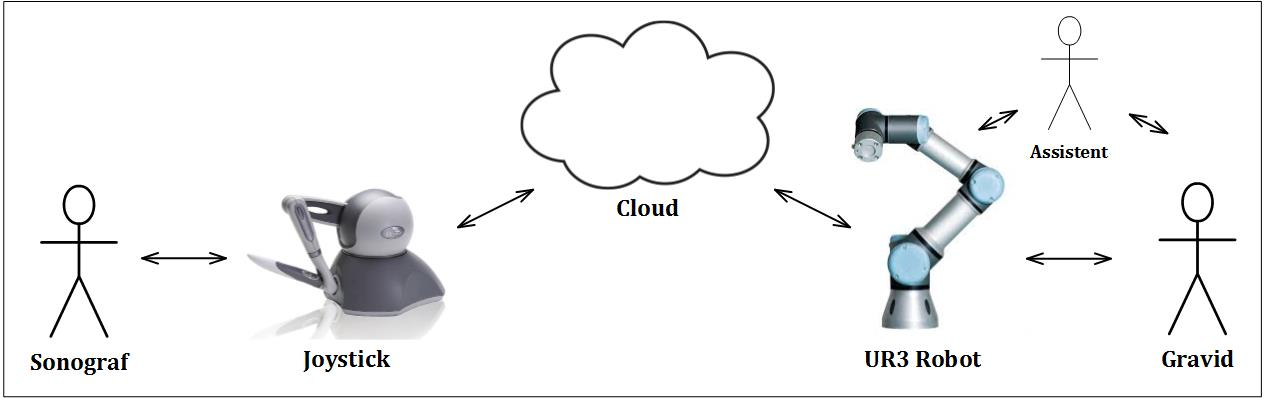
\includegraphics[width = 1.0\textwidth]{Figurer/teknologiTelemedicin.jpg}
	\caption{Sammenhæng mellem systemets dele ved ændring til en telemedicinsk robotarm.}
	\label{systemTelemedicin}
\end{figure}

I Grønland er der få steder, hvor ultralydsscanninger kan udføres og derved store afstande mellem de gravide og sonograferne. Her vil den telemedicinske udgave bevirke, at en sonograf i Danmark, eller et andet sted i Grønland, kan foretage scanningen på gravide placeret afsides steder i Grønland. Dette vil give besparinger på transportudgifter, da patienterne såvel som sonograferne, ikke længere skal transporteres over store afstande ved de rutinemæssige scanninger, se Bilag 12, 18.02.2016. 
Dette vil ligeledes være til gavn i Danmark, hvor ultralydsscanninger vil kunne blive udført i provinserne, selvom sonograferne er placeret i de større byer. Derfor er der potentiale både internationalt og nationalt, da sonografen fra sin egen afdeling vil kunne tilbyde sin ekspertise på tværs af afdelingerne på landets hospitaler. 

Ultralyds Robotarmen som telemedicinsk udgave underbygges af studier, som har undersøgt brugen af ultralyds robotarme som telemedicinske løsninger. Studierne inden for telemedicinsk ultralydsscanning har været i gang i en årrække. Studierne undersøger, hvorvidt det er muligt at få samme kvalitet på telemedicinske scanninger som ved manuelle scanninger. Det undersøges, om billedkvaliteten forbliver den samme, når data skal sendes over internettet. Yderligere undersøges det, om den telemedicinske scanning kan foretages tilfredsstillende \cite{8}\cite{5}\cite{18}\cite{Hjerterobot}. 






\chapter{Referencer}
			%Skal den være der i sidste ende? 

\chapter{Bilag}
\begin{enumerate}
\item Datablad Universal Robots UR3
\item Brochure til Universal Robots UR3
\item Datablad til joystick Geomagic Touch
\item Interview med HEH
\item Interview med RMV
\item Mailkorrespondance med Søren Pallesne
\item Mailkorrespondance med HEH
\item Mailkorrespondance med RMV
\item Mailkorrespondance med Skejby
\item Dansk Føtalmedicinsk Selskab Guidelines
\item Søgeprotokol
\end{enumerate}



\backmatter
\bibliography{bibliografi/Ref}    % Sætter bibliografien bagerst i dokumentet. Bruger bib-filen PRJ3.
\newpage
%\listoffigures	%Figurliste
%\listoftables	%Liste over alle tabeller

\end{document}
